\chapter{Program Verification}\label{ch:hoare}

Testing can show the presence of bugs but not their absence. \emph{Formal verification}
proves that a program meets its specification for \emph{all} inputs. We use Floyd--Hoare
logic for a small imperative language, as in Huth and Ryan.

\section{The programming language}

Programs (commands) $C$ are built from integer expressions $E$ and Boolean expressions $B$:
\[
C ::= x = E \;\mid\; C_1;\,C_2 \;\mid\; \code{if}\ (B)\ \{C_1\}\ \code{else}\ \{C_2\}
      \;\mid\; \code{while}\ (B)\ \{C\}
\]
Expressions are side-effect free (they always terminate and do not change variables), and
variables hold unbounded integers. Later we add arrays.

\section{Hoare triples}

\begin{definition}[Hoare triple]
A \emph{Hoare triple} $\hoare{P}{C}{Q}$ consists of a \emph{precondition} $P$, a program
$C$, and a \emph{postcondition} $Q$, where $P,Q$ are first-order formulas over the
program variables (and arithmetic).
\begin{itemize}
  \item $\hoare{P}{C}{Q}$ is satisfied under \emph{partial correctness}, written
        $\pc\hoare{P}{C}{Q}$, if for every state satisfying $P$, \emph{if} $C$
        terminates, the final state satisfies $Q$.
  \item It is satisfied under \emph{total correctness}, written $\tc\hoare{P}{C}{Q}$, if
        for every state satisfying $P$, $C$ \emph{is guaranteed to terminate} and the
        final state satisfies $Q$.
\end{itemize}
\end{definition}

Total correctness = partial correctness + termination.

\begin{center}
\begin{tikzpicture}[>=Stealth,font=\small]
  \draw[fill=blue!6] (0,0) ellipse (1.3cm and 1.5cm);
  \draw[fill=green!8] (6,0) ellipse (1.3cm and 1.5cm);
  \node at (0,1.8) {states satisfying $P$};
  \node at (6,1.8) {states satisfying $Q$};
  \foreach \y in {0.7,0} {\fill (0.2,\y) circle (1.5pt); \fill (5.8,\y-0.1) circle (1.5pt);
    \draw[->] (0.2,\y) to[bend left=8] node[above,font=\scriptsize]{$C$} (5.8,\y-0.1);}
  \fill (0.1,-0.8) circle (1.5pt);
  \draw[->,red!60!black,decorate,decoration={coil,aspect=0.6,segment length=6pt,amplitude=3pt}] (0.1,-0.8) -- (3.2,-1.3);
  \node[font=\scriptsize,red!60!black,anchor=west] at (3.25,-1.35) {never terminates};
\end{tikzpicture}

\small Partial correctness only constrains the runs that end; total correctness also forbids the
non-terminating one.
\end{center}

\begin{example}
\begin{itemize}
  \item $\hoare{x=5}{y = x+1}{y=6}$ holds (partially and totally).
  \item $\hoare{\top}{\code{while (true) \{ x = x \}}}{x = 42}$ holds under partial
        correctness (vacuously: it never terminates) but not total correctness.
  \item $\hoare{\top}{y = x\cdot x}{y > 0}$ fails: $x=0$ gives $y=0$.
\end{itemize}
\end{example}

\begin{important}[Logical variables]
Specifications often need to refer to initial values. Use \emph{logical variables}
(which the program never assigns), e.g.\
$\hoare{x=x_0\land y=y_0}{C_{\mathrm{swap}}}{x=y_0\land y=x_0}$.
Also beware trivial ``solutions'': $\hoare{x\ge0}{y=1;\ x=0}{y=x!}$ is correct because the
postcondition did not pin down $x$. Use logical variables to prevent this.
\end{important}

\section{Proof rules for partial correctness}

\renewcommand{\arraystretch}{1.3}
\begin{center}
\begin{tabular}{ll}
Assignment &
 $\dfrac{}{\hoare{Q[E/x]}{x = E}{Q}}$\\[3ex]
Composition &
 $\dfrac{\hoare{P}{C_1}{R}\qquad\hoare{R}{C_2}{Q}}{\hoare{P}{C_1;C_2}{Q}}$\\[3ex]
If-statement &
 $\dfrac{\hoare{P\land B}{C_1}{Q}\qquad\hoare{P\land\neg B}{C_2}{Q}}
        {\hoare{P}{\code{if}\ (B)\ \{C_1\}\ \code{else}\ \{C_2\}}{Q}}$\\[3ex]
Partial-while &
 $\dfrac{\hoare{I\land B}{C}{I}}{\hoare{I}{\code{while}\ (B)\ \{C\}}{I\land\neg B}}$\\[3ex]
Implied (consequence) &
 $\dfrac{\vdash P\to P'\qquad\hoare{P'}{C}{Q'}\qquad\vdash Q'\to Q}{\hoare{P}{C}{Q}}$
\end{tabular}
\end{center}
\renewcommand{\arraystretch}{1}

\subsection{The assignment rule}

The assignment rule works \emph{backwards}: to have $Q$ after $x=E$, we need $Q$ with $E$
in place of $x$ before. It looks backwards at first but is correct; the ``obvious''
forward version $\hoare{P}{x=E}{P[E/x]}$ is wrong (try $\hoare{x=2}{x=3}{3=2}$).

\begin{example}
\begin{itemize}
  \item $\hoare{y+1=6}{x = y+1}{x=6}$, and $y+1=6$ simplifies to $y=5$.
  \item $\hoare{x+1>0}{x = x+1}{x>0}$: the precondition is $x>-1$, i.e.\ $x\ge0$.
  \item $\hoare{2\cdot 3 = 6}{x = 3}{2x=6}$: the precondition is a tautology.
\end{itemize}
\end{example}

\subsection{Proof tableaux}

Rather than write proof trees, we annotate the program, interleaving code and assertions.
Each assertion is justified by the rule that produced it; adjacent assertions with no code
between them must be related by an implication (justified by ``implied'', with a separate
proof of that implication in ordinary maths or natural deduction). We usually fill a
tableau in \emph{from the bottom up}, pushing the postcondition backwards through
assignments.

\begin{example}[Swap with a temporary]
\leavevmode\begin{center}
\begin{tabular}{@{}l@{\qquad}l@{}}
$\{x=x_0\land y=y_0\}$ & \\
$\{y=y_0\land x=x_0\}$ & implied\\
\code{t = x;} & \\
$\{y=y_0\land t=x_0\}$ & assignment\\
\code{x = y;} & \\
$\{x=y_0\land t=x_0\}$ & assignment\\
\code{y = t;} & \\
$\{x=y_0\land y=x_0\}$ & assignment
\end{tabular}
\end{center}
Reading upward: substitute $t$ for $y$, then $y$ for $x$, then $x$ for $t$.
\end{example}

\begin{example}[Maximum]
\leavevmode\begin{center}
\begin{tabular}{@{}l@{\qquad}l@{}}
$\{\top\}$ & \\
\code{if (x > y) \{} & \\
\quad$\{\top\land x>y\}$ & if-statement\\
\quad$\{x=\max(x,y)\}$ & implied\\
\quad\code{m = x;} & \\
\quad$\{m=\max(x,y)\}$ & assignment\\
\code{\} else \{} & \\
\quad$\{\top\land\neg(x>y)\}$ & if-statement\\
\quad$\{y=\max(x,y)\}$ & implied\\
\quad\code{m = y;} & \\
\quad$\{m=\max(x,y)\}$ & assignment\\
\code{\}} & \\
$\{m=\max(x,y)\}$ & if-statement
\end{tabular}
\end{center}
\end{example}

\section{Loops and invariants}

\begin{definition}[Loop invariant]
A \emph{loop invariant} for \code{while (B) \{C\}} is a formula $I$ such that
$\pc\hoare{I\land B}{C}{I}$: if $I$ holds at the start of an iteration (and the guard is
true), it holds again at the end.
\end{definition}

To prove $\hoare{P}{\code{while (B) \{C\}}}{Q}$ we need an $I$ with
\begin{enumerate}
  \item $P\to I$ \quad(the invariant holds initially);
  \item $\hoare{I\land B}{C}{I}$ \quad(it is preserved by the body);
  \item $I\land\neg B\to Q$ \quad(on exit it gives the postcondition).
\end{enumerate}

\begin{center}
\begin{tikzpicture}[>=Stealth,font=\small,node distance=0.55cm,
  as/.style={draw,rounded corners,fill=yellow!10,minimum height=0.6cm},
  cmd/.style={draw,fill=blue!5,minimum height=0.6cm,minimum width=1.4cm},
  test/.style={draw,diamond,aspect=2,inner sep=1pt,fill=gray!8}]
  \node[as] (p) {$P$};
  \node[as,below=of p] (i) {$I$};
  \node[test,below=of i] (b) {$B$?};
  \node[cmd,right=2cm of b] (c) {$C$};
  \node[as,below=of b] (ib) {$I\land\neg B$};
  \node[as,below=of ib] (q) {$Q$};
  \draw[->] (p) -- node[left,font=\scriptsize]{(1) $P\to I$} (i);
  \draw[->] (i) -- (b);
  \draw[->] (b) -- node[above,font=\scriptsize]{true} (c);
  \draw[->] (c) |- node[pos=0.25,right,font=\scriptsize]{(2) $\hoare{I\land B}{C}{I}$} (i);
  \draw[->] (b) -- node[left,font=\scriptsize]{false} (ib);
  \draw[->] (ib) -- node[left,font=\scriptsize]{(3) $I\land\neg B\to Q$} (q);
\end{tikzpicture}
\end{center}

\begin{important}[Finding invariants]
\begin{itemize}
  \item Trace the loop on a small input and tabulate variable values at the start of each
        iteration; look for a relationship that stays constant.
  \item The invariant usually ``generalises'' the postcondition by replacing a constant
        (like $x$ or $n$) by the loop counter. E.g.\ post $y=x!$ suggests $y=z!$.
  \item It must be strong enough that $I\land\neg B\to Q$, but weak enough to be true
        initially and preserved. Often an extra conjunct (like $z\le x$) is needed.
\end{itemize}
\end{important}

\begin{example}[Factorial]
Program \code{Fac1}: compute $y=x!$.
\begin{center}
\begin{tabular}{@{}l@{\qquad}l@{}}
$\{x\ge0\}$ & \\
$\{1=0!\}$ & implied\\
\code{y = 1;} & \\
$\{y=0!\}$ & assignment\\
\code{z = 0;} & \\
$\{y=z!\}$ & assignment\\
\code{while (z != x) \{} & \\
\quad$\{y=z!\land z\ne x\}$ & partial-while\\
\quad$\{y\cdot(z+1)=(z+1)!\}$ & implied\\
\quad\code{z = z + 1;} & \\
\quad$\{y\cdot z=z!\}$ & assignment\\
\quad\code{y = y * z;} & \\
\quad$\{y=z!\}$ & assignment\\
\code{\}} & \\
$\{y=z!\land\neg(z\ne x)\}$ & partial-while\\
$\{y=x!\}$ & implied
\end{tabular}
\end{center}
The invariant is $I \equiv y=z!$. The implied steps: $1=0!$ is true; $y=z!\to
y(z+1)=(z+1)!$ by the definition of factorial; $y=z!\land z=x\to y=x!$.
\end{example}

\begin{example}[Sum $1+\dots+n$]
\leavevmode\begin{center}
\begin{tabular}{@{}l@{\qquad}l@{}}
$\{n\ge0\}$ & \\
$\{0=\sum_{k=1}^{0}k\land 0\le n\}$ & implied\\
\code{s = 0; i = 0;} & \\
$\{s=\sum_{k=1}^{i}k\land i\le n\}$ & assignment (twice)\\
\code{while (i < n) \{} & \\
\quad$\{s=\sum_{k=1}^{i}k\land i\le n\land i<n\}$ & partial-while\\
\quad$\{s+i+1=\sum_{k=1}^{i+1}k\land i+1\le n\}$ & implied\\
\quad\code{i = i + 1;} & \\
\quad$\{s+i=\sum_{k=1}^{i}k\land i\le n\}$ & assignment\\
\quad\code{s = s + i;} & \\
\quad$\{s=\sum_{k=1}^{i}k\land i\le n\}$ & assignment\\
\code{\}} & \\
$\{s=\sum_{k=1}^{i}k\land i\le n\land\neg(i<n)\}$ & partial-while\\
$\{s=\sum_{k=1}^{n}k\}$ & implied
\end{tabular}
\end{center}
Here the conjunct $i\le n$ is essential: without it, $\neg(i<n)$ gives only $i\ge n$, not
$i=n$.
\end{example}

\section{Total correctness}

Partial correctness ignores termination. Since only \code{while} loops can fail to
terminate in our language, we strengthen the while rule.

\begin{definition}[Variant]
A \emph{variant} (ranking function) for a loop is an integer expression $V$ such that
\begin{itemize}
  \item $I\land B\to V\ge0$ (it is non-negative whenever the body is about to run), and
  \item each execution of the body strictly decreases $V$.
\end{itemize}
Since a non-negative integer cannot decrease forever, the loop terminates.
\end{definition}

\[
\text{Total-while:}\qquad
\dfrac{\hoare{I\land B\land 0\le V=v_0}{C}{I\land 0\le V<v_0}}
      {\hoare{I\land 0\le V}{\code{while}\ (B)\ \{C\}}{I\land\neg B}}
\]
where $v_0$ is a fresh logical variable recording the variant's value at the start of
the iteration. The other rules are the same as for partial correctness.

\begin{example}[Total correctness of \code{Fac1}]
Use invariant $I\equiv y=z!\land z\le x$ and variant $V\equiv x-z$. Initially $z=0\le x$
by the precondition $x\ge0$. In the body, $z\le x\land z\ne x$ gives $z<x$, so
$V=x-z>0$; after $z=z+1$ the new variant is $x-z-1<v_0$ and still $\ge0$. Note that
without the precondition $x\ge0$ the loop runs forever on negative $x$, so only partial
correctness would hold.
\end{example}
\begin{center}
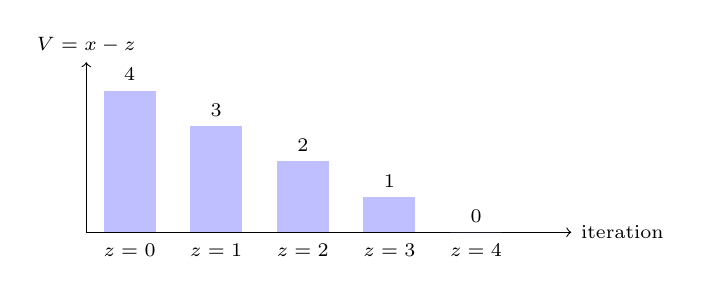
\begin{tikzpicture}[x=1.1cm,y=0.45cm,font=\small]
  \draw[->] (0,0) -- (5.6,0) node[right,font=\scriptsize]{iteration};
  \draw[->] (0,0) -- (0,4.8) node[above,font=\scriptsize]{$V=x-z$};
  \foreach \k in {0,...,4} {
    \pgfmathtruncatemacro\v{4-\k}
    \fill[blue!25] (\k+0.2,0) rectangle (\k+0.8,\v);
    \node[font=\scriptsize] at (\k+0.5,-0.5) {$z=\k$};
    \node[font=\scriptsize] at (\k+0.5,\v+0.45) {$\v$};
  }
\end{tikzpicture}

\small For $x=4$ the variant drops by one each iteration and the loop exits when it reaches $0$.
\end{center}

\begin{important}[Pitfalls]
\begin{itemize}
  \item Do not forget that the invariant must hold \emph{before} the loop, so the
        initialisation code is part of the proof.
  \item Every pair of adjacent assertions needs an ``implied'' justification that is
        actually a valid implication; check them separately.
  \item Variants must be integers bounded below; ``$x$ gets smaller'' over the reals does
        not guarantee termination.
\end{itemize}
\end{important}

\section{Arrays}

An array assignment \code{a[i] = E} changes the whole array value $a$. We model arrays as
functions and write $a\{i\leftarrow e\}$ for the array that agrees with $a$ except at
index $i$, where it has value $e$:
\[
(a\{i\leftarrow e\})[j]=\begin{cases}e & \text{if } j=i,\\ a[j] & \text{if } j\ne i.\end{cases}
\]
\[
\text{Array assignment:}\qquad \dfrac{}{\hoare{Q[a\{i\leftarrow E\}/a]}{a[i] = E}{Q}}
\]

\begin{example}[Aliasing]
What precondition guarantees $\{a[j]=3\}$ after \code{a[i] = 3}? By the rule,
$(a\{i\leftarrow3\})[j]=3$, which simplifies (case split on $i=j$) to
$i=j\lor a[j]=3$. Naively treating $a[i]$ like a separate variable would give just
$a[j]=3$ and miss the case where $i$ and $j$ are the same index.
\end{example}

\begin{example}[Sum of an array]
\leavevmode\begin{center}
\begin{tabular}{@{}l@{\qquad}l@{}}
$\{n\ge0\}$ & \\
\code{s = 0; i = 0;} & \\
$\{s=\sum_{k=0}^{i-1}a[k]\land 0\le i\le n\}$ & assignment, implied\\
\code{while (i < n) \{} & \\
\quad$\{s=\sum_{k=0}^{i-1}a[k]\land 0\le i\le n\land i<n\}$ & partial-while\\
\quad$\{s+a[i]=\sum_{k=0}^{i}a[k]\land 0\le i+1\le n\}$ & implied\\
\quad\code{s = s + a[i];} & \\
\quad$\{s=\sum_{k=0}^{i}a[k]\land 0\le i+1\le n\}$ & assignment\\
\quad\code{i = i + 1;} & \\
\quad$\{s=\sum_{k=0}^{i-1}a[k]\land 0\le i\le n\}$ & assignment\\
\code{\}} & \\
$\{s=\sum_{k=0}^{n-1}a[k]\}$ & partial-while, implied
\end{tabular}
\end{center}
With variant $n-i$ this is also totally correct. The array is only read, so the plain
assignment rule suffices; the array rule is needed when the program writes to $a$ (e.g.\
in-place reversal or sorting, where the invariant typically says ``$a[0..i-1]$ is sorted
and is a permutation of the original'').
\end{example}

The invariant of the array sum, pictured at the start of an iteration:
\begin{center}
\begin{tikzpicture}[>=Stealth,cell/.style={draw,minimum width=1.1cm,minimum height=0.6cm,font=\small}]
  \node[cell,fill=blue!12] (c0) at (0,0) {$a[0]$};
  \node[cell,fill=blue!12,right=0pt of c0] (c1) {$\cdots$};
  \node[cell,fill=blue!12,right=0pt of c1] (c2) {$a[i{-}1]$};
  \node[cell,right=0pt of c2] (c3) {$a[i]$};
  \node[cell,right=0pt of c3] (c4) {$\cdots$};
  \node[cell,right=0pt of c4] (c5) {$a[n{-}1]$};
  \draw[decorate,decoration={brace,amplitude=5pt}] (c0.north west) -- (c2.north east) node[midway,above=6pt,font=\small]{already added: $s=\sum_{k=0}^{i-1}a[k]$};
  \draw[<-] (c3.south) -- ++(0,-0.6) node[below,font=\small]{$i$};
\end{tikzpicture}
\end{center}

\section*{Summary}
\begin{itemize}
  \item $\pc\hoare{P}{C}{Q}$: if $P$ holds and $C$ terminates, $Q$ holds;
        $\tc$ additionally requires termination.
  \item Assignment works backwards: $\hoare{Q[E/x]}{x=E}{Q}$; build tableaux bottom-up.
  \item Loops need an invariant $I$: $P\to I$, $\hoare{I\land B}{C}{I}$,
        $I\land\neg B\to Q$.
  \item Termination: a non-negative integer variant that strictly decreases each iteration.
  \item Arrays: treat \code{a[i]=E} as assigning the updated array $a\{i\leftarrow E\}$;
        watch for aliasing.
\end{itemize}
